%!TEX program = xelatex
%!BIB program = bibtex
\documentclass[cn,black,12pt,normal]{elegantnote}
\usepackage{float}
\usepackage{hyperref}
\usepackage{amsmath}
\usepackage{amsfonts}
\usepackage{amssymb}
\usepackage{siunitx}[=v2]
\usepackage{fancyhdr}
\usepackage{newtxtext}
\usepackage{algorithm}
\usepackage{algorithmic}
\newcommand{\uct}[1]{\textsuperscript{\textsuperscript{\cite{#1}}}}
\renewcommand{\tablename}{\textbf{Table}}
\renewcommand{\figurename}{Figure.}
\renewcommand{\refname}{References}
\renewcommand{\contentsname}{Contents}
\renewcommand{\versiontext}{Version: }
\renewcommand{\updatetext}{Update: }
\PassOptionsToPackage{no-math}{fontspec}
\lstset{basicstyle=\footnotesize\ttfamily\color[RGB]{50,0,130},numbers=none,frame=trBL}

\sisetup{mode=text}
\sisetup{range-phrase = \text{ \textasciitilde }}
\pagestyle{fancy}
\fancyhead[L]{School of Software Engineering, Tongji University}
\fancyhead[R]{Data Structure Projects}
\renewcommand{\headrulewidth}{1pt}

\title{Electrical grid\\电网建设造价模拟系统}
\author{1951510\; 姜文渊}
\institute{\small \url{https://github.com/jwyjohn/Jwy_DataStructureHomework}}
\version{0.50}
\date{\today}

\begin{document}

\maketitle

\section{Introduction}

Suppose in a city, there are many communities that need to be powered by a electrical grid. Due to limited budget, the network should cost as little as possible. Here we have the estimated cost for connecting two certain communities, and the author need to implement an algorithm for giving out the optimized plan for the construction of such electrical grid.

Graph is useful in modeling real world problems, and in this situation, the problem is equivalent to the construction of a minimum spanning tree in an undirected graph.

A minimum spanning tree (MST) or minimum weight spanning tree is a subset of the edges of a connected, edge-weighted undirected graph that connects all the vertices together, without any cycles and with the minimum possible total edge weight. That is, it is a spanning tree whose sum of edge weights is as small as possible.\uct{wiki:Minimum_spanning_tree}

Several algorithms can be used to solve such problems. The Prim's algorithm\uct{cheriton1976finding} is one of the widely used one, and another popular algorithm is Kruskal's algorithm\uct{kruskal1956shortest}. Both the two algorithms costs $O(m\, log\, n)$ time, but faster algorithm are still invented recently.

The author implemented the Prim's algorithm in this project, considering its relatively fast speed and robustness.


\section{Demostration}

\subsection{Compile and run the program}

On linux platform with \lstinline{make} and a \lstinline{g++} which supports C++ 11 Standard, just \lstinline{cd} to the \lstinline{./linux} and run \lstinline{make build}. The binary executable will be generated in the same dirctory named as \lstinline{a.out} or \lstinline{egrid}, according to the configurations in the \lstinline{Makefile}. Use \lstinline{./a.out} to run the program.

The program is an interactive shell, where you can input commands and get results.

\begin{figure}[H]
    \centering
    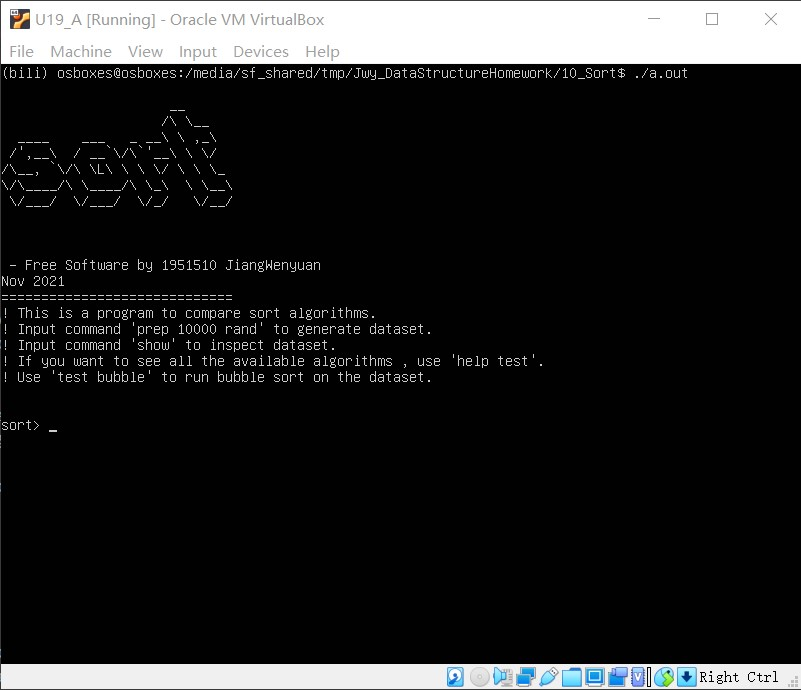
\includegraphics[width=0.7\linewidth]{image/sort_01.jpg}
    \caption{The user interface of the program}
\end{figure}

Usage of commands can be found on the main screen, and the \lstinline{help} command can give you information about theses commands.  All available commands is listed below.

\begin{enumerate}
    \item \lstinline{help} : Show help for a certain command.
    \item \lstinline{exit} : Exit the program.
    \item \lstinline{prep [N] (rand/seq/inv)} : Generate the data for sorting, where \lstinline{[N]} is an integer $> 10$ and $< 1000000$ (the limits depend on your conf and platform).
    \item \lstinline{show} : Show your full dataset.
    \item \lstinline{test (default/bubble/selection/insertion/binsertion/shell/quick/heap/bucket/merge/lsd/msd)} : Run certain sort algorithm and show its performance.
    \item \lstinline{seed} : Show the random seed used in this run.
\end{enumerate}

\subsection{Generate the data for testing sort algorithms}

Type \lstinline{prep 10000 rand} to generate a sequence from 1 to 10000 and randomly suffule them as our dataset for sorting.

\begin{figure}[H]
    \centering
    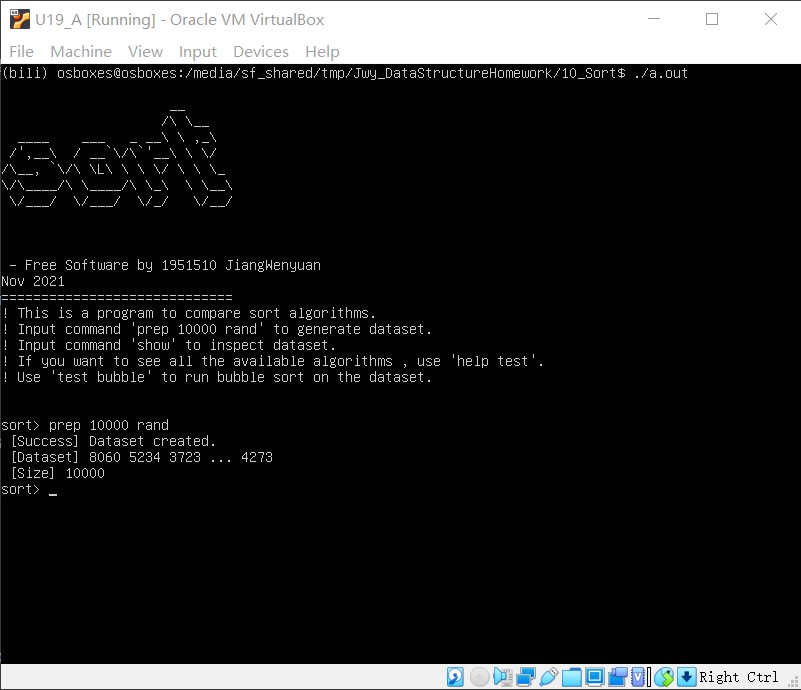
\includegraphics[width=0.7\linewidth]{image/sort_02.jpg}
    \caption{Use \lstinline{prep 10000 rand} to generate dataset (seed: \lstinline{1636865632})}
\end{figure}

To examine our dataset, use \lstinline{show}.

\begin{figure}[H]
    \centering
    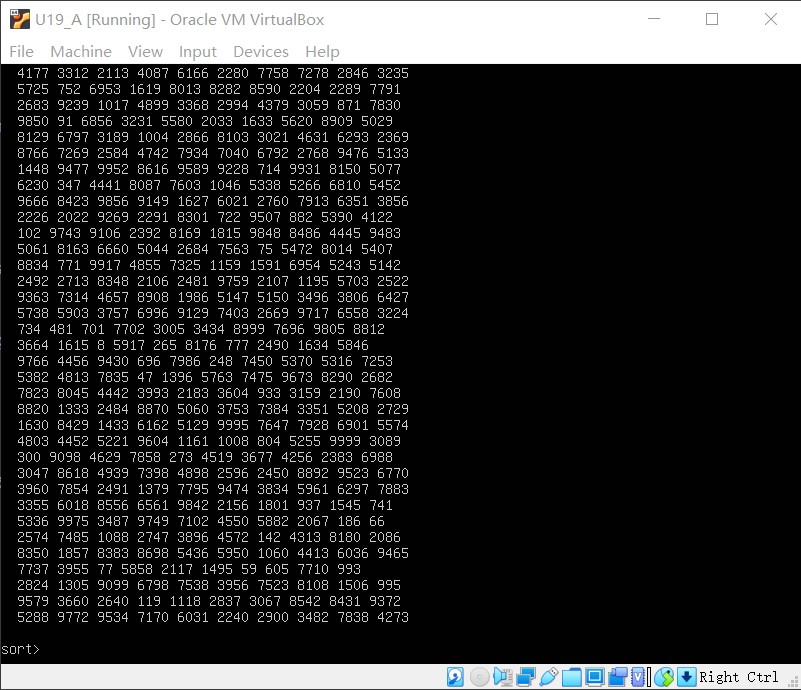
\includegraphics[width=0.7\linewidth]{image/sort_03.jpg}
    \caption{Use \lstinline{show} to view our dataset}
\end{figure}

\subsection{Run an algorithm}

Type \lstinline{test merge} to run Merge Sort on the generated dataset, the results and the performance indicators (Compare func calls, Swap calls and clocks used) will be shown.

\begin{figure}[H]
    \centering
    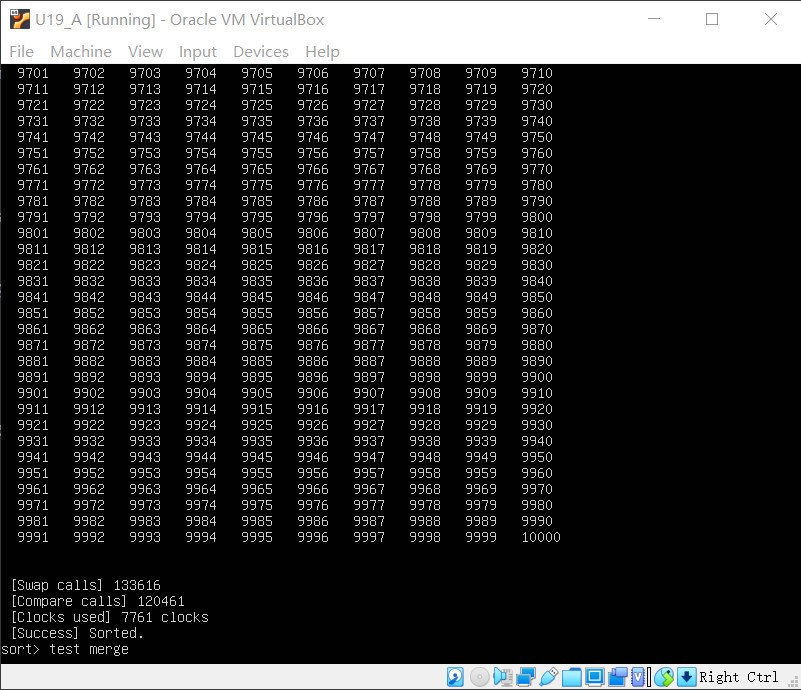
\includegraphics[width=0.7\linewidth]{image/sort_04.jpg}
    \caption{Use \lstinline{test} to run a sort}
\end{figure}

\section{Theoretical comparison of algorithms}

On many data structure or algorithm textbooks, it has been proved that comparison-based sorting algorithms have a fundamental requirement of $\Omega(n \, log \, n) $ comparisons,\uct{cormen2009introduction} whlie those sort methods not based on comparisons, such as Bucket Sort, can have better performance at a cost of more space.

Here we consider Computational complexity (best, average and worst), memory usage and stability of these Sort Algorithms, and the results are shown in the table below. Detailed proof can be found on various papers or textbooks.

\begin{table}[H]
    \caption{\textbf{Theoretical comparison of algorithms}}
    \centering
    \begin{tabular}{cccccc}
        \toprule
        Algorithm             & Best            & Average           & Worst             & Memory     & Stable \\
        \midrule
        Bubble Sort           & $n$             & $n^2$             & $n^2$             & $1$        & Yes    \\
        Insertion Sort        & $n$             & $n^2$             & $n^2$             & $1$        & Yes    \\
        Selection Sort        & $n^2$           & $n^2$             & $n^2$             & $1$        & Yes    \\
        Binary insertion Sort & $n$             & $n^2$             & $n^2$             & $1$        & Yes    \\
        Shell Sort            & $n \, log \, n$ & $n^{\frac{4}{3}}$ & $n^{\frac{3}{2}}$ & 1          & No     \\
        Quick Sort            & $n \, log \, n$ & $n \, log \, n$   & $n^2$             & $log \, n$ & No     \\
        Heap Sort             & $n \, log \, n$ & $n \, log \, n$   & $n \, log \, n$   & $1$        & No     \\
        Merge Sort            & $n \, log \, n$ & $n \, log \, n$   & $n \, log \, n$   & $n$        & Yes    \\
        Bucket sort           & $n$             & $n$               & $n$               & $n$        & Yes    \\
        Radix Sort            & $-$             & $nr$              & $nr$              & $n$        & Yes    \\
        \bottomrule
    \end{tabular}
\end{table}

Note that even though these algorithms are named as sorts, some of them have more wider application with minor modification. For exapmle, Heap Sort can be adjusted to maintain a priority queue with high performance. Some of the sort algorithms seems to be of low efficiency, but they have their value in theory or in some special cases. Another thing that needs to be mentioned about these algorithms is that, in the era of big data, paralle computation is more important than ever. One of the highly parallelizable sort algorithms is the Merge Sort, which can run on clusters.\uct{ajtai19830}


\section{Notes on the source code}

If you want to re-use the author's source code in a project, it is not recommended to do so for that the \lstinline{std::sort} is averagely more fast and more stable than these algorithms for testing.

But still, some of these algorithms are fun to test. In the author's source code \lstinline{main_header.h}, you can find a definition of a struct \lstinline{sort_func_result} like this:
\begin{lstlisting}[language = C++]
struct sort_func_result
{
	string func_name;
	int swap_count, compare_count;
};
\end{lstlisting}
This struct is used for showing the sort function name and some performance indicators. Implementation of different sorting algorithms are a function with return type as \lstinline{sort_func_result}. One example is the \lstinline{heap_sort}:
\begin{lstlisting}[language = C++]
sort_func_result heap_sort(int *array, int array_size, bool (*cmp)(int a, int b))
{
	sort_func_result ret;
	ret.func_name = __FUNCTION__;
	int swap_count = 0, cmp_count = 0;
	int last_non_leaf_node = array_size / 2 - 1;
	init_counter();
	int heap[array_size];
	int heap_size = array_size;
	for (int i = 0; i < array_size; i++)
		heap[i] = array[i];
	for (int i = last_non_leaf_node; i >= 0; i--)
	{
......
\end{lstlisting}
Note that the parameters of \lstinline{heap_sort} are \lstinline{int *array, int array_size, bool (*cmp)(int a, int b)}, where \lstinline{cmp} is a bool function for returning the result of comparing two values.

Detailed implementation of each algorithm follows the textbooks used in this course, and the comments in the code may help you understand how each algorithm actually works. Most of the code in \lstinline{main.cpp} is for processing the user's input, which is not so interesting.


\section{Results}



\section{Discussion}

\bibliography{references}
\end{document}
